Im ersten Aufgabenteil wird eine Referenzspannung von $U_\text{ref}=6.56 \;\si{\volt}$
und eine Signalspannung von $U_\text{sig}=13.5 \;\si{\volt}$ angelegt.
Die Frequenz wird hierbei manuell reguliert und die Spannungsamplituden
$U_\text{SS}$ werden peak-to-peak gemessen. Für die Messwerte in Tabelle \ref{tab:b}
wird ein Gain von 100 verwendet, für die Werte in Tabelle \ref{tab:d} wird ein Gain
von 1000 verwendet. Die Folgenden Werte sind bereits von diesen Verstärkungen bereinigt.


\begin{table}[!h]
  \centering
  % \begin{subtable}{0.3\textwidth}
  %   \begin{tabular}{S[table-format=4.0]S}
  %     \toprule
  %     {$\varphi$} &
  %     {$U_\text{SS} \,/\, \si{\volt}$} \\
  %     \midrule
  %     15\si{\degree} & 0.82  \\
  %     45\si{\degree} & 0.81 \\
  %     105\si{\degree} & 0.46  \\
  %     165\si{\degree} & 0.88 \\
  %     225\si{\degree} & 0.82  \\
  %     330\si{\degree}  & 0.83  \\
  %     \bottomrule
  %   \end{tabular}
  %   \caption{ohne Tiefpass}
  %   \label{tab:a}
  % \end{subtable}
  % \quad
  % \begin{subtable}{0.3\textwidth}
    \begin{tabular}{S[table-format=4.0]SS}
      \toprule
      {$\Delta\varphi$} &
      {$U_\text{max} \,/\, \si{\volt}\cdot10^{-3}$} &
      {$U_\text{out} \,/\, \si{\volt}\cdot10^{-3}$} \\
      \midrule
    -105\si{\degree}    &    -5     &     -3.18 \\
     -90\si{\degree}    &     5     &      3.07 \\
     -75\si{\degree}    &    25     &     13.78 \\
     -60\si{\degree}    &    45     &     20.27 \\
     -15\si{\degree}    &    80     &      0.00 \\
      15\si{\degree}    &    78     &     24.83 \\
      30\si{\degree}    &    65     &    -29.26 \\
      60\si{\degree}    &    20     &    -12.30 \\
      75\si{\degree}    &    5      &     -3.18 \\
     105\si{\degree}    &    -25    &     13.78 \\
     120\si{\degree}    &    -53    &     23.86 \\
     150\si{\degree}    &    -80    &     13.18 \\
    \bottomrule
    \end{tabular}
    \caption{Messwerte ohne Rauschen, mit Tiefpass}
    % \caption{mit Tiefpass}
    \label{tab:b}
  % \end{subtable}
  \quad
  \hfill
\end{table}


\begin{table}[!h]
  \centering
% \begin{subtable}{0.3\textwidth}
%   \begin{tabular}{S[table-format=4.0]S}
%     \toprule
%     {$\varphi$} &
%     {$U_\text{SS} \,/\, \si{\milli\volt}$} \\
%     \midrule
%     0\si{\degree}   & 88.0  \\
%     120\si{\degree} & 56.8  \\
%     165\si{\degree} & 92.0  \\
%     240\si{\degree} & 67.2  \\
%     270\si{\degree} & 48.8  \\
%     315\si{\degree} & 70.4  \\
%     \bottomrule
%   \end{tabular}
%   \caption{ohne Tiefpass}
%   \label{tab:c}
% \end{subtable}
% \quad
% \begin{subtable}{0.3\textwidth}
  \begin{tabular}{S[table-format=4.0]SS}
    \toprule
    {$\Delta\varphi$} &
    {$U_\text{max} \,/\, \si{\volt}\cdot10^{-4}$} &
    {$U_\text{out} \,/\, \si{\volt}\cdot10^{-4}$} \\
    \midrule
  -105  \si{\degree}  &    0     &      0.00 \\
   -90  \si{\degree}  &    5     &      3.07 \\
   -75  \si{\degree}  &    16    &      8.82 \\
   -60  \si{\degree}  &    35    &     15.76 \\
   -15  \si{\degree}  &    50    &      0.00 \\
    15  \si{\degree}  &    46    &    -14.64 \\
    30  \si{\degree}  &    38    &    -17.11 \\
    60  \si{\degree}  &    10    &     -6.15 \\
    75  \si{\degree}  &    1     &     -0.64 \\
   105  \si{\degree}  &    -20   &     11.03 \\
   120  \si{\degree}  &    -35   &     15.76 \\
   150  \si{\degree}  &    -50   &      8.24 \\
    \bottomrule
  \end{tabular}
  \caption{Messwerte mit Rauschen, Signal Attenuator = 1,
          Noise Amplitude = 1$\times 10^{-3}$, mit Tiefpass}
  % \caption{mit Tiefpass}
  \label{tab:d}
% \end{subtable}
\quad
\hfill
\end{table}

Die Werte für $U_\text{out}$ lassen sich mit Hilfe der Formel \eqref{eqn:out} berechnen.\\
\newpage

\begin{figure}[!h]
\begin{minipage}[t]{0.3\textwidth}
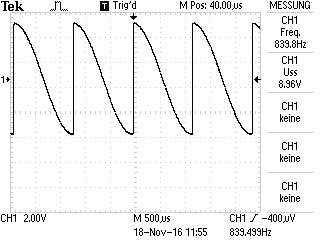
\includegraphics[width=\textwidth]{Bilder/15.jpg}
\caption{$\varphi = 15\si{\degree}$}
\label{fig:1}
\end{minipage}
\hspace{10pt}
\vspace{5pt}
\begin{minipage}[t]{0.3\textwidth}
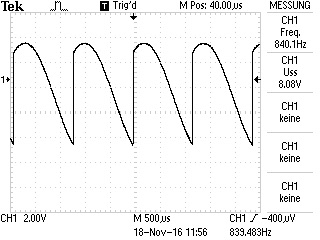
\includegraphics[width=\textwidth]{Bilder/45.jpg}
\caption{$\varphi = 45\si{\degree}$}
\label{fig:2}
\end{minipage}
\hspace{10pt}
\vspace{5pt}
\begin{minipage}[t]{0.3\textwidth}
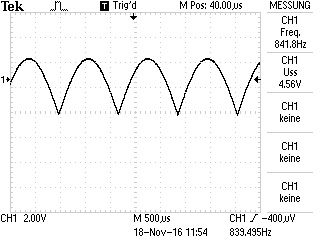
\includegraphics[width=\textwidth]{Bilder/105.jpg}
\caption{$\varphi = 105\si{\degree}$}
\label{fig:3}
\end{minipage}
\hspace{10pt}
\vspace{5pt}
\begin{minipage}[t]{0.3\textwidth}
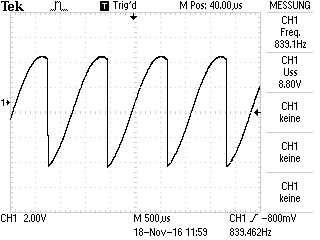
\includegraphics[width=\textwidth]{Bilder/165.jpg}
\caption{$\varphi = 165\si{\degree}$}
\label{fig:4}
\end{minipage}
\hspace{12pt}
\vspace{5pt}
\begin{minipage}[t]{0.3\textwidth}
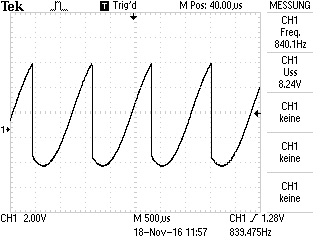
\includegraphics[width=\textwidth]{Bilder/225.jpg}
\caption{$\varphi = 225\si{\degree}$}
\label{fig:5}
\end{minipage}
\hspace{12pt}
\vspace{5pt}
\begin{minipage}[t]{0.3\textwidth}
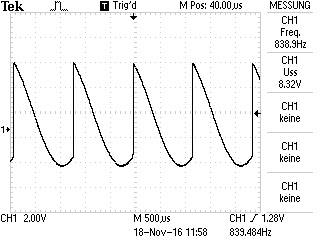
\includegraphics[width=\textwidth]{Bilder/330.jpg}
\caption{$\varphi = 330\si{\degree}$}
\label{fig:6}
\end{minipage}
\hspace{12pt}
\vspace{5pt}
\end{figure}

In den Abbildungen \ref{fig:1} bis \ref{fig:6} sind die Spannungskurven für unterschiedliche Phasen
zu sehen. Hierbei wird weder der Tiefpassfilter noch der Rausch-Generator eingeschaltet. \\
Abbildung \ref{fig:1} zeigt eine sehr steile positive Flanke und spitze Extrema. Abbildung \ref{fig:2}
zeigt auch sehr steile positive Flanken, jedoch sind die Hochpunkte abgerundet. In Abbildung \ref{fig:3}
sieht der Verlauf ungefähr wie der Betrag der Sinus-Kurve aus. In Abbildung \ref{fig:4}
ist die negative Flanke sehr steil, die Hochpunkte sind abgerundet und die Tiefpunkte spitz.
Der Graph in Abbildung \ref{fig:5} hat sehr spitze Hochpunkte und eine sehr steile negative Flanke.
Der Graph in der letzten Abbildung \ref{fig:6} sieht aus wie der Graph aus Abbildung \ref{fig:5}, nur
das er an der y-Achse gespiegelt ist.

\newpage

\begin{figure}[!h]
\begin{minipage}[t]{0.3\textwidth}
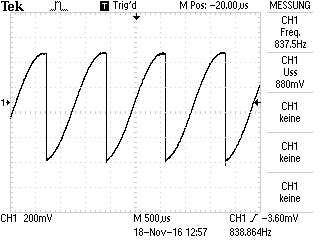
\includegraphics[width=\textwidth]{Bilder/Rausch0.jpg}
\caption{$\varphi = 0\si{\degree}$}
\label{fig:7}
\end{minipage}
\hspace{10pt}
\vspace{5pt}
\begin{minipage}[t]{0.3\textwidth}
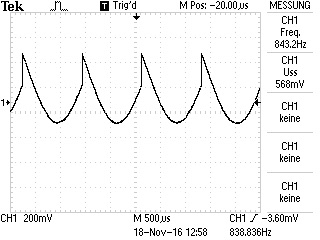
\includegraphics[width=\textwidth]{Bilder/Rausch120.jpg}
\caption{$\varphi = 120\si{\degree}$}
\label{fig:8}
\end{minipage}
\hspace{10pt}
\vspace{5pt}
\begin{minipage}[t]{0.3\textwidth}
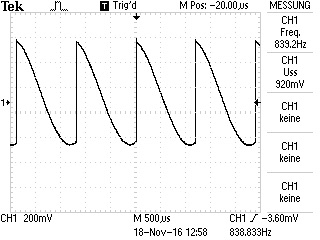
\includegraphics[width=\textwidth]{Bilder/Rausch165.jpg}
\caption{$\varphi = 165\si{\degree}$}
\label{fig:9}
\end{minipage}
\hspace{10pt}
\vspace{5pt}
\begin{minipage}[t]{0.3\textwidth}
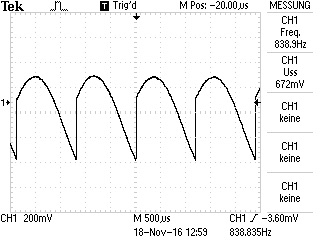
\includegraphics[width=\textwidth]{Bilder/Rausch240.jpg}
\caption{$\varphi = 240\si{\degree}$}
\label{fig:10}
\end{minipage}
\hspace{12pt}
\vspace{5pt}
\begin{minipage}[t]{0.3\textwidth}
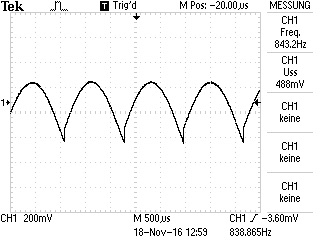
\includegraphics[width=\textwidth]{Bilder/Rausch270.jpg}
\caption{$\varphi = 270\si{\degree}$}
\label{fig:11}
\end{minipage}
\hspace{12pt}
\vspace{5pt}
\begin{minipage}[t]{0.3\textwidth}
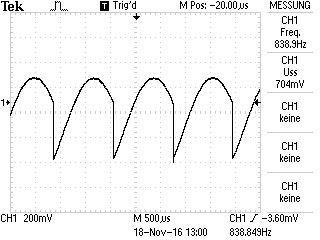
\includegraphics[width=\textwidth]{Bilder/Rausch315.jpg}
\caption{$\varphi = 315\si{\degree}$}
\label{fig:12}
\end{minipage}
\hspace{12pt}
\vspace{5pt}
\end{figure}

In den Abbildungen \ref{fig:7} bis \ref{fig:12} sind die Spannungskurven mit
eingeschaltetem Rausch-Generator zu sehen. Der Tiefpassfilter ist weiterhin ausgeschaltet. \\

\newpage

Im zweiten Teil der Auswertung wird die Abhängigkeit der Ausgangsspannung zur Phasenverschiebung
betrachtet. Hier wird sowohl mit, als auch ohne Rausch-Generator gemessen. Zur besseren
Darstellung wird $\cos{(\Delta\varphi)}$ gegen die gemessenen Werte $U_\text{max}$
geplottet. Diese Werte sind in Tabelle \ref{tab:b} einzusehen.

\begin{figure}[H]
  \centering
  \includegraphics[width=1.0\textwidth]{Bilder/phi.pdf}
  \caption{$U_\text{max}$ in Abhängigkeit von $\cos{(\Delta\varphi)}$.}
  \label{fig:Umax}
\end{figure}
Mit Python ergibt sich für den ersten Graphen
\begin{align*}
  a &= (82 ± 5) \mV   \\
  b &= (-3 ± 3) \mV
\end{align*}
und für den zweiten Graphen
\begin{align*}
  a &= (51 ± 5) \,\cdot 10^{-1} \, \mV      \\
  b &= (-2 ± 3) \,\cdot 10^{-1} \, \mV
\end{align*}.

\newpage


Im letzten Teil der Auswertung wird untersucht, bei welcher maximalen Entfernung $r$
eine Photodiode keinen Lichtimpuls einer LED mehr aufnimmt. Dabei wird die eingehende Spannung $U$
gegen den Abstand $r$ mit den Messdaten aus Tabelle \ref{tab:licht} geplottet.
Zu Beginn wird eine Dunkelmessung durchgeführt, welche einen Wert von $U = 0.06 \,\mV$
ergibt. Dieser Wert wird bei den aufgenommenen Spannungswerten im Folgenden direkt
abgezogen. Zudem werden die Werte mit einer Low-Pass Verstärkung von 50, einem
Pre-Amplifier von 2 und einer Lock-In Verstärkung von 2 aufgenommen. Im Folgenden
sind die Messwerte jedoch schon von diesen Verstärkungen bereinigt.

\begin{table}[H]
  \centering
    \begin{tabular}{cccc}
      \toprule
      {$r \,/ \cm$} & {$U \, / \mV$} & {$r \,/\cm$} & {$U \,/ \mV$} \\
      \midrule
       0  &  2.100   &   22  &  0.125 \\
       2  &  1.200   &   24  &  0.125 \\
       4  &  0.775   &   26  &  0.100 \\
       6  &  0.525   &   28  &  0.100 \\
       8  &  0.375   &   30  &  0.100 \\
      10  &  0.300   &   32  &  0.100 \\
      12  &  0.250   &   34  &  0.075 \\
      14  &  0.200   &   36  &  0.075 \\
      16  &  0.150   &   38  &  0.075 \\
      18  &  0.150   &   40  &  0.075 \\
      20  &  0.125   &  \hrulefill     &  \hrulefill      \\
      \bottomrule
    \end{tabular}
    \caption{Messwerte des Abstands der LED/PD Messung}
    \label{tab:licht}
\end{table}

\begin{figure}[H]
  \centering
  \includegraphics[width=\textwidth]{Bilder/Plot_Photodiode.pdf}
  \caption{U in Abhängigkeit von r}
  \label{fig:led}
\end{figure}

In Grafik \ref{fig:led} ist zu erkennen, dass die Spannung exponentiell zum Abstand
abnimmt. Daraus folgt:

\begin{equation*}
  U \propto \frac{1}{r^2}
\end{equation*}
Der Graph wird mit
\begin{equation}
U = a + \frac{b}{(r+c)^2} \notag
\end{equation}
gefittet.
Dabei ergeben sich die Parameter:
\begin{align*}
  a &= (-0.027 ± 0.005) \; \si{\milli\volt} \\
  b &= (69 ± 2)    \;   \si{\milli\volt\cdot\centi\square\meter}        \\
  c &= (-4.2 ± 0.1) \; \si{\centi\meter}
\end{align*}
\\
Nun wird die Ausgangsspannung gegen $1/r^2$ geplottet, damit ein linearer Fit mit ipython durchgeführt
werden kann.

\begin{figure}[!h]
\centering
\includegraphics[width=\textwidth]{Bilder/photo.pdf}
\caption{Lineare Regression}
\label{fig:lin}
\end{figure}

Die Parameter der Ausgleichgeraden in Grafik \ref{fig:lin} lauten:

\begin{align*}
    a &= (194 ± 9) \; \si{\milli\volt\per\square\centi\meter} \\
    b &= (-0.14 ± 0.03) \; \si{\milli\volt}
\end{align*}
